\documentclass[10pt, aspectratio=54]{beamer}
\usetheme{Boadilla}
\usefonttheme{serif} 
\setbeamertemplate{background canvas}{}
\definecolor{customblue}{RGB}{0, 102, 204}
\setbeamercolor{title}{fg=customblue}
\setbeamercolor{frametitle}{fg=customblue}
\setbeamertemplate{itemize item}{\color{customblue}$\blacksquare$}
\usepackage[utf8]{inputenc}
\usepackage[english]{babel}
\usepackage{algorithm}
\usepackage{algorithmic}
\usepackage{amsmath}
\usepackage{amsfonts}
\usepackage{amssymb}
\usepackage{ragged2e}
\usepackage{graphicx}

\usepackage{listings}
\usepackage{xcolor}

% Define custom style for Python code
\lstdefinestyle{mystyle}{
	backgroundcolor=\color{gray!10},   % light gray background
	commentstyle=\color{gray!100},
	keywordstyle=\color{blue},
	stringstyle=\color{red},
	basicstyle=\ttfamily\fontsize{8}{8}\selectfont, % Typewriter font and small size
	breaklines=true,                   % Automatic line breaking
	frame=single,                      % Adds a frame around the code
}

% Apply the style to Python code
\lstset{style=mystyle}

\graphicspath{{./Figures/}}

\author{Petar Bosnic}
\title{FDM Part 1: Vibration ODEs}
\subtitle{Numerical Solutions of Differential Equations}
\setbeamercovered{transparent}
\institute[]{PhD Student, \\ Department of Process, Energy and Environmental Technology \\ Faculty of Technology, Natural Sciences and Maritime Sciences \\ University of South-Eastern Norway,\\ Campus Porsgrunn} 
\date{12/09/2024}

\begin{document}
	
	\begin{frame}
		\titlepage
	\end{frame}

	
%	\begin{frame}{Table of Contents}
%		\tableofcontents
%	\end{frame}
	
	\begin{frame}{Overview of Presentation}
		\justifying
		This presentation will cover the following key topics:
		\begin{itemize}
			\item \textbf{Introduction to FDM:} Basic principles of the Finite Difference Method (FDM).
			\item \textbf{Numerical Schemes:} Detailed discussion of numerical schemes for solving vibration ODEs.
			\item \textbf{Example Problem:} Step-by-step solution of a simple vibration problem using FDM.
			\item \textbf{Simulation Algorithm:} Construction of algorithms for simulation and analysis.
			\item \textbf{Verification and Validation:} Testing the accuracy and stability of the FDM implementation.
			\item \textbf{Generalization:} Extending FDM to solve more complex vibration problems.
			\item \textbf{Applications of Vibration Models:} Real-world applications of FDM in engineering and making code open-source (GitHub).
			\item \textbf{Open-source:} Making code open-source on GitHub.
		\end{itemize}
	\end{frame}
	
	
	\begin{frame}{Finite Difference Method: Overview and basic concept}
		\justifying
%		Overview and basic concept behind Finite Difference Method (FDM).
		
		\begin{minipage}{0.5\textwidth}
			\flushleft
			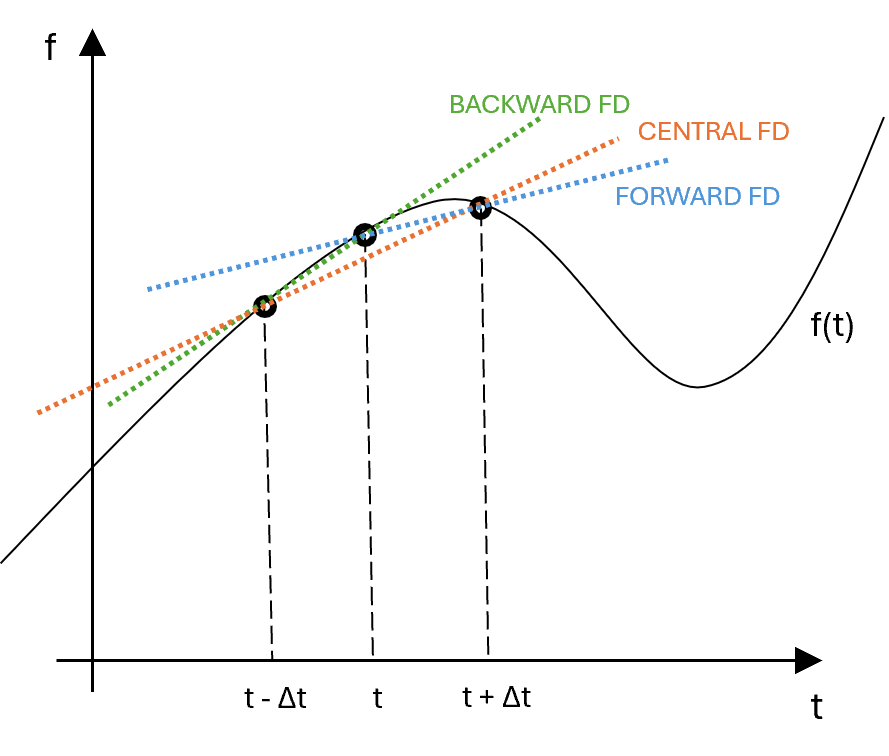
\includegraphics[width=\textwidth]{Figures/FDM.png}
		\end{minipage}
		\hfill
		\begin{minipage}{0.45\textwidth}
			\centering
			\textbf{First order derivative:} 
			\[
			\frac{d f(t)}{d t} = \lim_{\Delta t \to 0} \frac{f(t + \Delta t) - f(t)}{\Delta t}
			\]
			\[
			\frac{d f(t)}{d t} \approx \frac{f(t + \Delta t) - f(t)}{\Delta t}
			\]
		\end{minipage}
		
		\vspace{0.3cm}
		
		% Taylor Expansion and Finite Difference Schemes
		\textbf{Taylor Expansion:}
		\[
		f(t + \Delta t) = f(t) + \frac{d f}{d t} \Delta t + \frac{d^2 f}{d t^2} \frac{\Delta t^2}{2!} + \frac{d^3 f}{d t^3} \frac{\Delta t^3}{3!} + O(\Delta t^4) + ...
		\]
		\[
		f(t - \Delta t) = f(t) - \frac{d f}{d t} \Delta t + \frac{d^2 f}{d t^2} \frac{\Delta t^2}{2!} - \frac{d^3 f}{d t^3} \frac{\Delta t^3}{3!} + O(\Delta t^4) - ...
		\]
				
	\end{frame}
	
	\begin{frame}{}
		\justifying
%		In this slide, we will present different finite difference schemes for approximating derivatives.
			% Taylor Expansion and Finite Difference Schemes
		\textbf{Taylor Expansion:}
		\[
		f(t + \Delta t) = f(t) + \frac{d f}{d t} \Delta t + \frac{d^2 f}{d t^2} \frac{\Delta t^2}{2!} + \frac{d^3 f}{d t^3} \frac{\Delta t^3}{3!} + O(\Delta t^4) + ...
		\]
		\[
		f(t - \Delta t) = f(t) - \frac{d f}{d t} \Delta t + \frac{d^2 f}{d t^2} \frac{\Delta t^2}{2!} - \frac{d^3 f}{d t^3} \frac{\Delta t^3}{3!} + O(\Delta t^4) - ...
		\]
		\textbf{Forward Difference Scheme:}
		\[
		\frac{d f}{d t} \approx \frac{f(t + \Delta t) - f(t)}{\Delta t} = \frac{d f}{d t} + \frac{d^2 f}{d t^2} \frac{\Delta t}{2!} + \frac{d^3 f}{d t^3} \frac{\Delta t^2}{3!} + ...
		\]
		
		\textbf{Backward Difference Scheme:}
		\[
		\frac{d f}{d t} \approx \frac{f(t) - f(t - \Delta t)}{\Delta t} =  \frac{d f}{d t} - \frac{d^2 f}{d t^2} \frac{\Delta t}{2!} + \frac{d^3 f}{d t^3} \frac{\Delta t^2}{3!} - ...
		\]
		
		\textbf{Central Difference Scheme:}
		\[
		\frac{d f}{d t} \approx \frac{f(t + \Delta t) - f(t - \Delta t)}{2\Delta t} =  \frac{d f}{d t} +  \frac{d^3 f}{d t^3} \frac{\Delta t^2}{3!} + \frac{d^4 f}{d t^4} \frac{\Delta t^3}{4!} + ...
		\]
	\end{frame}
	
	\begin{frame}{}
		\justifying
		\textbf{Second Order Derivative:}
		\[
		\frac{d^2 f(t)}{d t^2} = \lim_{\Delta t \to 0} \frac{f'(t + \Delta t) - f'(t)}{\Delta t}
		\]
		Using the central difference scheme, we approximate the second derivative by combining forward and backward Taylor expansions.
		
		\vspace{0.3cm}
		
		\textbf{Taylor Expansion:}
		\[
		f(t + \Delta t) = f(t) + \frac{d f}{d t} \Delta t + \frac{d^2 f}{d t^2} \frac{\Delta t^2}{2!} + \frac{d^3 f}{d t^3} \frac{\Delta t^3}{3!} + O(\Delta t^4)
		\]
		\[
		f(t - \Delta t) = f(t) - \frac{d f}{d t} \Delta t + \frac{d^2 f}{d t^2} \frac{\Delta t^2}{2!} - \frac{d^3 f}{d t^3} \frac{\Delta t^3}{3!} + O(\Delta t^4)
		\]
		
		\vspace{0.3cm}
		
		\textbf{Central Difference Approximation:}
		\[
		\frac{d^2 f(t)}{d t^2} \approx \frac{f(t + \Delta t) - 2f(t) + f(t - \Delta t)}{\Delta t^2} + O(\Delta t^2)
		\]
	\end{frame}


	\begin{frame}{Vibration Problem Setup}
		\centering
		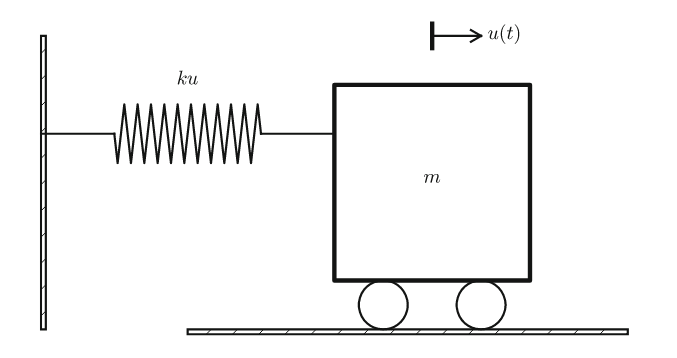
\includegraphics[width=0.5\textwidth]{Figures/Vibrating_system_scheme.png} % Adjust the width to fit the slide
		
		
		We aim to solve the following second-order differential equation using the central difference method:
		\[
		u''(t) + \omega^2 u(t) = 0
		\]
		\textbf{Initial Conditions:}
		\begin{itemize}
			\item \( u(0) = I \)  \quad (initial displacement)
			\item \( u'(0) = 0 \) \quad (initial velocity)
		\end{itemize}
		\textbf{Time Domain:} \( t \in [0, T] \)
		
		\vspace{0.3cm}
		The goal is to approximate the displacement \( u(t) \) at discrete time steps using the central difference method.
	\end{frame}
	
	\begin{frame}{Central Difference Method}
		\justifying
		The central difference method approximates the second-order derivative of \( u(t) \) using the formula:
		\[
		u''(t_n) \approx \frac{u(t_{n+1}) - 2u(t_n) + u(t_{n-1})}{\Delta t^2}
		\]
		Substituting this into the vibration equation \( u''(t) + \omega^2 u(t) = 0 \), we get:
		\[
		\frac{u(t_{n+1}) - 2u(t_n) + u(t_{n-1})}{\Delta t^2} + \omega^2 u(t_n) = 0
		\]
		Solving for \( u(t_{n+1}) \):
		\[
		u(t_{n+1}) = 2u(t_n) - u(t_{n-1}) - \omega^2 \Delta t^2 u(t_n)
		\]
	\end{frame}
	
	\begin{frame}{Discretization of Time}
		\justifying
		We discretize the time domain into \( N \) equally spaced intervals with time step \( \Delta t \):
		\[
		t_n = n \Delta t \quad \text{where} \quad n = 0, 1, 2, \ldots, N
		\]
		\textbf{Time Step Size:}
		\[
		\Delta t = \frac{T}{N}
		\]
		At each time step \( t_n \), we compute the displacement \( u(t_n) \) using the central difference formula.
	\end{frame}
	
	\begin{frame}{Applying Initial Conditions}
		\justifying
		To start the solution process, we need the values of \( u \) at the first two time steps.
		\begin{itemize}
			\item From the initial condition, \( u(0) = I \).
			\item For \( u'(0) = 0 \), we use a central difference approximation for the first derivative:
			\[
			u'(0) \approx \frac{u(1) - u(-1)}{2\Delta t} = 0 \quad \Rightarrow \quad u(-1) = u(1) 
			\]

		\end{itemize}

	\end{frame}
	
	\begin{frame}{Recursive Solution}
		\justifying
		Using the central difference method, we compute \( u(t_{n+1}) \) recursively:
		\[
		u(t_{n+1}) = 2u(t_n) - u(t_{n-1}) - \omega^2 \Delta t^2 u(t_n)
		\]
		The algorithm proceeds as follows:
		\begin{itemize}
			\item Initialize \( u(0) = I \) and \( u(1) = I - 0.5  \omega^2 \Delta t^2 u(0)\)
			\item For each subsequent time step \( t_n \), compute \( u(t_{n+1}) \) using the formula
		\end{itemize}
		Continue until \( t = T \).
	\end{frame}
	
	\begin{frame}[fragile]{Python Implementation}
		
\begin{lstlisting}[language=Python]
def u_exact(t, I, w):
  return I * np.cos(w * t)

def solver(I, w, dt, T):
  dt = float(dt)            # Ensure dt is a float
  Nt = int(round(T / dt))   # Number of time steps
  u = np.zeros(Nt + 1)      # Solution array initialized to zero
  t = np.linspace(0, Nt * dt, Nt + 1)  # Time array
	
  u[0] = I     # Initial condition u(0) = I
	
  # Central Difference Method
  u[1] = I - 0.5 * w**2 * u[0] * dt**2  # u'(0) = 0
	
  for n in range(1, Nt):
    u[n+1] = 2 * u[n] - u[n-1] - w**2 * u[n] * dt**2
	
  return u, t
\end{lstlisting}	
	\end{frame}
	
\begin{frame}[fragile]{Visualization and Main Function}
	\justifying
	The following Python functions handle the visualization of the numerical solution compared to the exact solution:
	
	\begin{lstlisting}[language=Python]
def visualize(u, t, I, w, dt, ax):
 # Generate a finer time grid and compute the exact solution 
 t_fine = np.linspace(0, t[-1], 1001)
 u_e = u_exact(t_fine, I, w)
 	
 # Plot the numerical and exact solutions
 ax.plot(t, u, 'r--x', label='Central Difference (CD)')
 ax.plot(t_fine, u_e, 'b-', label='Exact Solution')
	
 ax.legend(loc='lower left')
 ax.set_xlabel('t')  # Label for the x-axis (time)
 ax.set_ylabel('u')  # Label for the y-axis (displacement)
 ax.set_title('dt = %g' % dt)  # Title indicating the time step size
 ax.set_xlim(t[0], t[-1])  # Set the limits for the x-axis (time)
	
 # Adjust layout to prevent overlap of plot elements
 plt.tight_layout()
		
	\end{lstlisting}
\end{frame}

\begin{frame}[fragile]{Visualization and Main Function}
	
	\begin{lstlisting}[language=Python]
# Main function to visualize the solutions for different dt
def main(I, w, dt_values, T):
 # Create a subplot for each time step value
 fig, axes = plt.subplots(len(dt_values), 1, figsize=(10, 10))
# Loop over each time step value
 for i, dt in enumerate(dt_values):
 # Solve the ODE using the central difference method
  u, t = solver(I, w, dt, T)
 # Visualize the numerical and exact solution
  visualize(u, t, I, w, dt, axes[i])
 # Display all the plots
 plt.show()
 
if __name__ == "__main__":
# User-defined parameters
I = 1.0           # Initial displacement
w = 2.0 * pi      # Angular frequency
num_periods = 5   # Number of oscillation periods to simulate
P = 2 * pi / w    # Calculate one period of the oscillation
T = P * num_periods  # Total time for the simulation
dt_values = [0.01, 0.1, 0.32]  # Different time steps to test

# Call the main function 
main(I, w, dt_values, T)
		
	\end{lstlisting}
\end{frame}


	
\begin{frame}{Visualization of Central Difference Method}
	\centering
	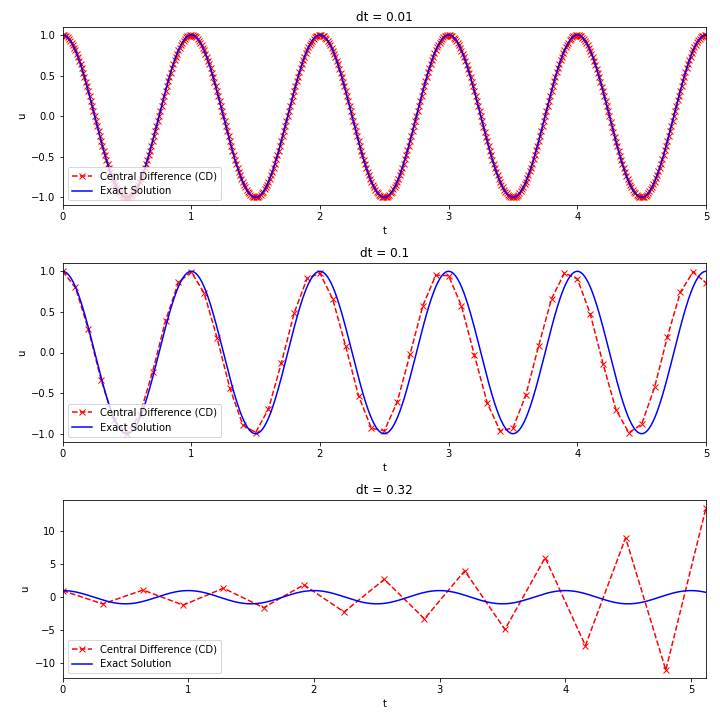
\includegraphics[width=0.7\textwidth]{Figures/CD_vib.png} % Adjust the width to fit the slide
\end{frame}


\begin{frame}[fragile]{Verification: Test Three Steps}
	
	\begin{lstlisting}[language=Python]
def test_three_steps():
  I = 1
  w = 2 * pi
  dt = 0.01
  T = 1
  # Expected result using exact solution (u_exact) for the first 3 steps
  t_exact = np.array([0, dt, 2*dt])
  u_by_hand = u_exact(t_exact, I, w)
	
  # Solve using the solver function
  u, t = solver(I, w, dt, T)
	
  # Compute the difference for the first three time steps
  diff = np.abs(u_by_hand - u[:3]).max()
	
  # Set tolerance
  tol = 1E-3
	
  # Assert that the difference is smaller than tolerance
  assert diff < tol, "Test failed: max difference {} exceeds tolerance {}".format(diff, tol)
	
  print("Test passed: max difference is {}".format(diff))
	\end{lstlisting}
\end{frame}

\begin{frame}[fragile]{Convergence Rates Function}
	
	\begin{lstlisting}[language=Python]
# Function to compute convergence rates
def convergence_rates(I, w, dt, T, m, solver_function, num_periods=8):
  dt_values = []
  E_values = []
  for i in range(m):
    u, t = solver_function(I, w, dt, T)
    u_e = u_exact(t, I, w)
    # Error estimation using L2 norm
    E = np.sqrt(dt * np.sum((u_e - u)**2))
    dt_values.append(dt)
    E_values.append(E)
    dt = dt / 2  # Halve the time step

  # Convergence rate calculation
  r = [np.log(E_values[i-1] / E_values[i]) /
  np.log(dt_values[i-1] / dt_values[i])
  for i in range(1, m)]
  return r, E_values, dt_values

	\end{lstlisting}
\end{frame}

\begin{frame}[fragile]{Convergence Rates Test Function}
	
	\begin{lstlisting}[language=Python]
def test_convergence_rates():
  I = 1.0
  w = 2.0 * pi
  num_periods = 8
  P = 2 * pi / w
  T = P * num_periods
  dt = P / 30
  m = 5
  # Run convergence rate test for the solver
  r, E, dt_values = convergence_rates(I, w, dt, T, m, solver)	
  # Set tolerance for the convergence rate (one decimal place)
  tol = 0.1	
  # Check if the last calculated convergence rate is approximately 2.0
  assert abs(r[-1] - 2.0) < tol, "Test failed: Convergence rate {} deviates from expected 2.0".format(r[-1])
  print("Solver convergence rates: {}".format(r))
  print("Test passed: Convergence rate {} is within tolerance {}".format(r[-1], tol))
		
	\end{lstlisting}
\end{frame}

\begin{frame}[fragile]{Test Output from Pytest}
	
	\begin{lstlisting}

=============== test session starts ================


CD_vib.py::test_three_steps Test passed: max difference is 2.59210806663e-06
PASSED
CD_vib.py::test_convergence_rates Solver convergence rates: [2.0036366687361946, 2.000949732812305, 2.0002401059790955, 2.0000601973344323]
Test passed: Convergence rate 2.00006019733 is within tolerance 0.1
PASSED

============== 2 passed in 0.35 seconds =============
	\end{lstlisting}
\end{frame}

\begin{frame}{Rewriting Second-Order ODE into First-Order System}
	\justifying
	To solve a second-order ODE numerically, we convert it into a system of first-order ODEs. Consider the second-order ODE:
	
	\[
	u''(t) + \omega^2 u(t) = 0
	\]
	
	\textbf{Step 1: Define new variables:}
	Let:
	\[
	v(t) = u'(t)
	\]
	Here, \( u(t) \) is the displacement and \( v(t) \) is the velocity.
	
	\textbf{Step 2: Express the second-order ODE as a system of first-order ODEs:}
	\[
	u'(t) = v(t)
	\]
	\[
	v'(t) = -\omega^2 u(t)
	\]
	
	
	\textbf{Conclusion:} The system is now a pair of first-order ODEs that can be solved numerically using methods such as Euler’s method, Crank-Nicolson, Euler-Cromer or Runge-Kutta methods.
\end{frame}

\begin{frame}{Forward Euler Method}
	\justifying
	The Forward Euler method solves the system using the following update scheme:
	
	\[
	u_{n+1} = u_n + \Delta t \cdot v_n
	\]
	\[
	v_{n+1} = v_n - \Delta t \cdot \omega^2 \cdot u_n
	\]
	
	\textbf{Algorithm:}
	\begin{enumerate}
		\item Initialize \( u_0 = I \), \( v_0 = 0 \).
		\item For each time step \( n \) from 0 to \( N-1 \):
		\[
		u_{n+1} = u_n + \Delta t \cdot v_n
		\]
		\[
		v_{n+1} = v_n - \Delta t \cdot \omega^2 \cdot u_n
		\]
	\end{enumerate}
\end{frame}

\begin{frame}{Backward Euler Method}
	\justifying
	The Backward Euler method is implicit and requires solving for \( v_{n+1} \) at each step:
	
	\[
	v_{n+1} = \frac{v_n - \Delta t \cdot \omega^2 \cdot u_n}{1 + \Delta t^2 \cdot \omega^2}
	\]
	\[
	u_{n+1} = u_n + \Delta t \cdot v_{n+1}
	\]
	
	\textbf{Algorithm:}
	\begin{enumerate}
		\item Initialize \( u_0 = I \), \( v_0 = 0 \).
		\item For each time step \( n \) from 0 to \( N-1 \):
		\[
		v_{n+1} = \frac{v_n - \Delta t \cdot \omega^2 \cdot u_n}{1 + \Delta t^2 \cdot \omega^2}
		\]
		\[
		u_{n+1} = u_n + \Delta t \cdot v_{n+1}
		\]
	\end{enumerate}
\end{frame}


\begin{frame}{Crank-Nicolson Method}
	\justifying
	The Crank-Nicolson method is semi-implicit and combines the forward and backward Euler methods:
	
	\[
	u_{n+1} = u_n + \Delta t \cdot v^*_n
	\]
	\[
	v_{n+1} = v_n - \Delta t \cdot \omega^2 \cdot u^*_n
	\]
	where \( u^*_n \) and \( v^*_n \) are intermediate values:
	\[
	u^*_n = u_n + 0.5 \cdot \Delta t \cdot v_n
	\]
	\[
	v^*_n = v_n - 0.5 \cdot \Delta t \cdot \omega^2 \cdot u_n
	\]
	
	\textbf{Algorithm:}
	\begin{enumerate}
		\item Initialize \( u_0 = I \), \( v_0 = 0 \).
		\item For each time step \( n \) from 0 to \( N-1 \):
		\[
		u^*_n = u_n + 0.5 \cdot \Delta t \cdot v_n
		\]
		\[
		v^*_n = v_n - 0.5 \cdot \Delta t \cdot \omega^2 \cdot u_n
		\]
		\[
		u_{n+1} = u_n + \Delta t \cdot v^*_n
		\]
		\[
		v_{n+1} = v_n - \Delta t \cdot \omega^2 \cdot u^*_n
		\]
	\end{enumerate}
\end{frame}

\begin{frame}{Runge-Kutta 2 Method (Heun's)}
	\justifying
	The RK2 method (Heun's method) uses two intermediate steps to improve accuracy:
	
	\[
	u_{n+1} = u_n + \frac{\Delta t}{2} (k_1^u + k_2^u)
	\]
	\[
	v_{n+1} = v_n + \frac{\Delta t}{2} (k_1^v + k_2^v)
	\]
	where:
	\[
	k_1^u = v_n, \quad k_1^v = -\omega^2 u_n
	\]
	\[
	u_{tilde} = u_n + \Delta t \cdot k_1^u, \quad v_{tilde} = v_n + \Delta t \cdot k_1^v
	\]
	\[
	k_2^u = v_{tilde}, \quad k_2^v = -\omega^2 u_{tilde}
	\]
	
	\textbf{Algorithm:}
	\begin{enumerate}
		\item Initialize \( u_0 = I \), \( v_0 = 0 \).
		\item For each time step \( n \) from 0 to \( N-1 \):
		\[
		k_1^u = v_n, \quad k_1^v = -\omega^2 u_n
		\]
		\[
		u_{tilde} = u_n + \Delta t \cdot k_1^u, \quad v_{tilde} = v_n + \Delta t \cdot k_1^v
		\]
		\[
		k_2^u = v_{tilde}, \quad k_2^v = -\omega^2 u_{tilde}
		\]
		\[
		u_{n+1} = u_n + \frac{\Delta t}{2} (k_1^u + k_2^u)
		\]
		\[
		v_{n+1} = v_n + \frac{\Delta t}{2} (k_1^v + k_2^v)
		\]
	\end{enumerate}
\end{frame}

%\begin{frame}{Runge-Kutta 4 Method}
%	\justifying
%	The Runge-Kutta 4 (RK4) method uses four intermediate steps for higher accuracy:
%	
%	\[
%	u_{n+1} = u_n + \frac{\Delta t}{6} (k_1^u + 2k_2^u + 2k_3^u + k_4^u)
%	\]
%	\[
%	v_{n+1} = v_n + \frac{\Delta t}{6} (k_1^v + 2k_2^v + 2k_3^v + k_4^v)
%	\]
%	where:
%	\[
%	k_1^u = v_n, \quad k_1^v = -\omega^2 u_n
%	\]
%	\[
%	k_2^u = v_n + 0.5 \Delta t k_1^v, \quad k_2^v = -\omega^2 \left( u_n + 0.5 \Delta t k_1^u \right)
%	\]
%	\[
%	k_3^u = v_n + 0.5 \Delta t k_2^v, \quad k_3^v = -\omega^2 \left( u_n + 0.5 \Delta t k_2^u \right)
%	\]
%	\[
%	k_4^u = v_n + \Delta t k_3^v, \quad k_4^v = -\omega^2 \left( u_n + \Delta t k_3^u \right)
%	\]
%	
%	\textbf{Algorithm:}
%	\begin{enumerate}
%		\item Initialize \( u_0 = I \), \( v_0 = 0 \).
%		\item For each time step \( n \) from 0 to \( N-1 \):
%		\[
%		k_1^u = v_n, \quad k_1^v = -\omega^2 u_n
%		\]
%		\[
%		k_2^u = v_n + 0.5 \Delta t k_1^v, \quad k_2^v = -\omega^2 \left( u_n + 0.5 \Delta t k_1^u \right)
%		\]
%		\[
%		k_3^u = v_n + 0.5 \Delta t k_2^v, \quad k_3^v = -\omega^2 \left( u_n + 0.5 \Delta t k_2^u \right)
%		\]
%		\[
%		k_4^u = v_n + \Delta t k_3^v, \quad k_4^v = -\omega^2 \left( u_n + \Delta t k_3^u \right)
%		\]
%		\[
%		u_{n+1} = u_n + \frac{\Delta t}{6} (k_1^u + 2k_2^u + 2k_3^u + k_4^u)
%		\]
%		\[
%		v_{n+1} = v_n + \frac{\Delta t}{6} (k_1^v + 2k_2^v + 2k_3^v + k_4^v)
%		\]
%	\end{enumerate}
%\end{frame}

\begin{frame}{Euler-Cromer Method}
	\justifying
	The Euler-Cromer method updates velocity first and then uses the updated velocity to compute displacement:
	
	\[
	v_{n+1} = v_n - \Delta t \cdot \omega^2 \cdot u_n
	\]
	\[
	u_{n+1} = u_n + \Delta t \cdot v_{n+1}
	\]
	
	\textbf{Algorithm:}
	\begin{enumerate}
		\item Initialize \( u_0 = I \), \( v_0 = 0 \).
		\item For each time step \( n \) from 0 to \( N-1 \):
		\[
		v_{n+1} = v_n - \Delta t \cdot \omega^2 \cdot u_n
		\]
		\[
		u_{n+1} = u_n + \Delta t \cdot v_{n+1}
		\]
	\end{enumerate}
\end{frame}

\begin{frame}{Implicit vs. Explicit Schemes}
	\justifying
	\textbf{Explicit Schemes:}
	\begin{itemize}
		\item Directly calculate the next time step based on known values from the current or previous steps.
	\end{itemize}
	
	\textbf{Implicit Schemes:}
	\begin{itemize}
		\item Involve solving an equation to calculate the next time step.
	\end{itemize}
	
	\vspace{0.3cm}
	\textbf{Table of Explicit and Implicit Schemes:}
	

		\centering
		\begin{tabular}{|p{3.5cm}|p{2cm}|p{5cm}|}
			\hline
			\textbf{Scheme}         & \textbf{Type}    & \textbf{Description}                \\ \hline
			Forward Euler           & Explicit         & Simple, first-order accurate        \\ \hline
			Central Difference      & Explicit         & Second-order accurate               \\ \hline
			Runge-Kutta (RK2, RK4)  & Explicit         & Higher-order accurate, multiple steps \\ \hline
			Backward Euler          & Implicit         & First-order accurate    \\ \hline
			Crank-Nicolson          & Implicit         & Second-order accurate\\ \hline
			Euler-Cromer            & Semi-Implicit    & First-order accurate, common in oscillatory systems       \\ \hline
		\end{tabular}

	
\end{frame}

\begin{frame}[fragile]{Numerical Solvers for ODEs for simple vibration system with multiple schemes}
	\scriptsize % Smaller font size for fitting the code
	\begin{lstlisting}[language=Python]
def solver(I, w, dt, T, method):
	dt = float(dt)
	Nt = int(round(T/dt))
	u = np.zeros(Nt + 1)
	t = np.linspace(0, Nt*dt, Nt+1)
	u[0] = I  # Initial condition u(0) = I

	if method == 'CD':  # Central Difference Method
	u[1] = I - 0.5 * w**2 * u[0] * dt**2  # u'(0) = 0
	for n in range(1, Nt):
		u[n+1] = 2 * u[n] - u[n-1] - w**2 * u[n] * dt**2
	
	elif method == 'FE':  # Forward Euler Method
	v = np.zeros(Nt + 1)
	v[0] = 0  # Initial velocity u'(0) = 0
	for n in range(Nt):
		u[n+1] = u[n] + dt * v[n]
		v[n+1] = v[n] - dt * w**2 * u[n]

	\end{lstlisting}
\end{frame}

\begin{frame}[fragile]{}
	\scriptsize % Smaller font size for fitting the code
	\begin{lstlisting}[language=Python]
	elif method == 'BE':  # Backward Euler Method
	v = np.zeros(Nt + 1)
	v[0] = 0  # Initial velocity u'(0) = 0
	for n in range(Nt):
		v[n+1] = (v[n] - dt * w**2 * u[n]) / (1 + dt**2 * w**2)
		u[n+1] = u[n] + dt * v[n+1]
	
	elif method == 'CN':  # Crank-Nicolson Method
	v = np.zeros(Nt + 1)
	v[0] = 0  # Initial velocity u'(0) = 0
	for n in range(Nt):
		u_star = u[n] + 0.5 * dt * v[n]
		v_star = v[n] - 0.5 * dt * w**2 * u[n]
		u[n+1] = u[n] + dt * v_star
		v[n+1] = v[n] - dt * w**2 * u_star
		
	elif method == 'EC':  # Euler-Cromer Method
		v = np.zeros(Nt + 1)
		v[0] = 0  # Initial velocity u'(0) = 0
		for n in range(Nt):
			if n == 0:
				v[1] = v[0] - 0.5*dt*w**2*u[n]
			else:
				v[n+1] = v[n] - dt * w**2 * u[n]
				u[n+1] = u[n] + dt * v[n+1]

		
	\end{lstlisting}
\end{frame}

\begin{frame}[fragile]{}
	\fontsize{5}{5}\selectfont
	\begin{lstlisting}[language=Python]
	elif method == 'RK2':  # Runge-Kutta 2 Method
		v = np.zeros(Nt + 1)
		v[0] = 0  # Initial velocity u'(0) = 0
		for n in range(Nt):
			k1_u = v[n]
			k1_v = -w**2 * u[n]
			u_tilde = u[n] + dt * k1_u
			v_tilde = v[n] + dt * k1_v
			k2_u = v_tilde
			k2_v = -w**2 * u_tilde
			u[n+1] = u[n] + 0.5 * dt * (k1_u + k2_u)
			v[n+1] = v[n] + 0.5 * dt * (k1_v + k2_v)
		
	elif method == 'RK4':  # Runge-Kutta 4 Method
		v = np.zeros(Nt + 1)
		v[0] = 0  # Initial velocity u'(0) = 0
		for n in range(Nt):
			k1_u = v[n]
			k1_v = -w**2 * u[n]
			k2_u = v[n] + 0.5 * dt * k1_v
			k2_v = -w**2 * (u[n] + 0.5 * dt * k1_u)
			k3_u = v[n] + 0.5 * dt * k2_v
			k3_v = -w**2 * (u[n] + 0.5 * dt * k2_u)
			k4_u = v[n] + dt * k3_v
			k4_v = -w**2 * (u[n] + dt * k3_u)
			u[n+1] = u[n] + (dt/6.0) * (k1_u + 2*k2_u + 2*k3_u + k4_u)
			v[n+1] = v[n] + (dt/6.0) * (k1_v + 2*k2_v + 2*k3_v + k4_v)

	return u, v, t		

	\end{lstlisting}
\end{frame}

\begin{frame}{Visualization of Different Methods: dt = 0.01}
	\centering
	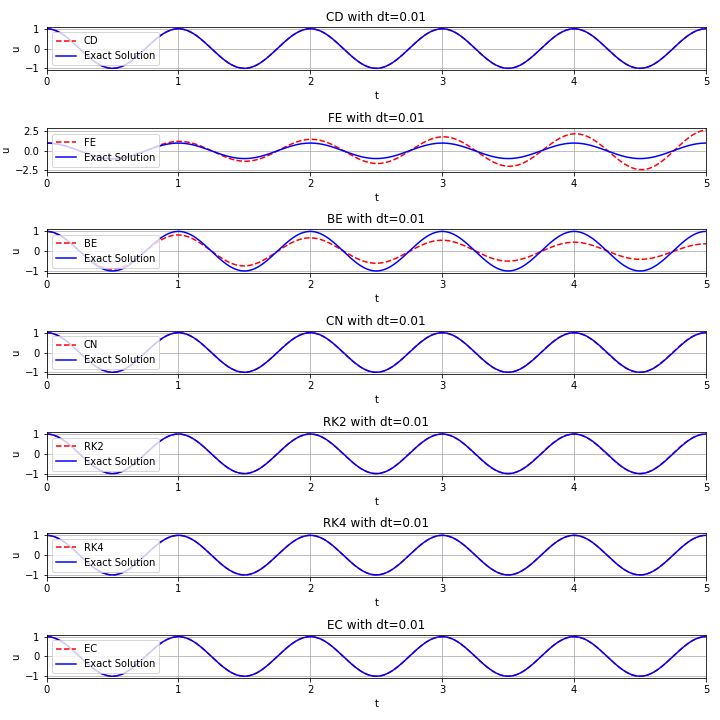
\includegraphics[width=0.7\textwidth]{Figures/Each_Method_Comparison_dt_0.01.png} % Adjust the width to fit the slide
\end{frame}
\begin{frame}{Visualization of Different Methods: dt = 0.1}
	\centering
	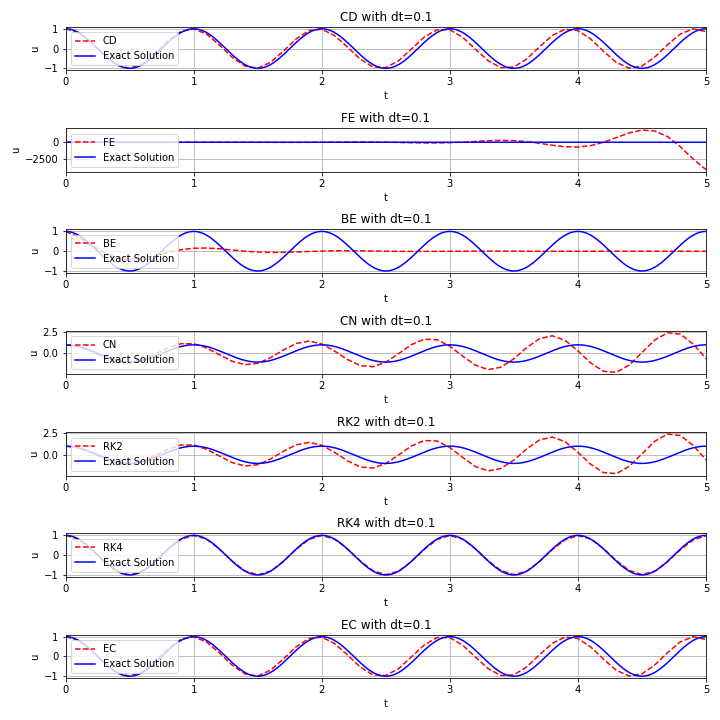
\includegraphics[width=0.7\textwidth]{Figures/Each_Method_Comparison_dt_0.1.png} % Adjust the width to fit the slide
\end{frame}

\begin{frame}[fragile]{Error and Convergence Test Results}
	\scriptsize % Adjust font size to fit the content on one slide
	
	\textbf{3-Step Error Test (dt = 0.01):}
	\begin{itemize}
		\item \textbf{Method CD:} PASSED. Max difference is 2.59e-06, expected [1.00, 0.9980, 0.9921], got [1.00, 0.9980, 0.9921].
		\item \textbf{Method FE:} FAILED (Difference: 0.00394, Tolerance: 0.001).
		\item \textbf{Method BE:} FAILED (Difference: 0.00388, Tolerance: 0.001).
		\item \textbf{Method CN:} PASSED. Max difference is 6.49e-06, expected [1.00, 0.9980, 0.9921], got [1.00, 0.9980, 0.9921].
		\item \textbf{Method RK2:} PASSED. Max difference is 6.49e-06, expected [1.00, 0.9980, 0.9921], got [1.00, 0.9980, 0.9921].
		\item \textbf{Method RK4:} PASSED. Max difference is 1.20e-09, expected [1.00, 0.9980, 0.9921], got [1.00, 0.9980, 0.9921].
		\item \textbf{Method EC:} PASSED. Max difference is 2.59e-06, expected [1.00, 0.9980, 0.9921], got [1.00, 0.9980, 0.9921].
	\end{itemize}
	
	\textbf{Error Convergence Test (dt = 0.01):}
	\begin{itemize}
		\item \textbf{Method CD:} PASSED. Convergence rate 2.0000 within tolerance 0.1.
		\item \textbf{Method FE:} FAILED. Convergence rate 1.0204 deviates from 2.0.
		\item \textbf{Method BE:} FAILED. Convergence rate 0.9808 deviates from 2.0.
		\item \textbf{Method CN:} PASSED. Convergence rate 2.0003 within tolerance 0.1.
		\item \textbf{Method RK2:} PASSED. Convergence rate 2.0003 within tolerance 0.1.
		\item \textbf{Method RK4:} FAILED. Convergence rate 4.0005 deviates from 2.0.
		\item \textbf{Method EC:} PASSED. Convergence rate 2.0000 within tolerance 0.1.
	\end{itemize}
	
	\textbf{Error Calculation (dt = 0.01):}
	\begin{itemize}
		\item \textbf{Method CD:} Global Error = 0.822483, Local Errors: [6.49e-07, 2.59e-06, 5.81e-06].
		\item \textbf{Method FE:} Global Error = 224.324891, Local Errors: [0.00197, 0.00394, 0.00587].
		\item \textbf{Method BE:} Global Error = 116.320050, Local Errors: [0.00196, 0.00388, 0.00574].
		\item \textbf{Method CN:} Global Error = 3.298773, Local Errors: [6.49e-07, 6.49e-06, 1.75e-05].
		\item \textbf{Method RK2:} Global Error = 3.298773, Local Errors: [6.49e-07, 6.49e-06, 1.75e-05].
		\item \textbf{Method RK4:} Global Error = 0.000651, Local Errors: [8.55e-11, 1.20e-09, 3.32e-09].
		\item \textbf{Method EC:} Global Error = 0.822483, Local Errors: [6.49e-07, 2.59e-06, 5.81e-06].
	\end{itemize}
\end{frame}


\begin{frame}[fragile]{Observations from Analysis}
	\begin{itemize}
		\item \textbf{Central Difference Method:} Performs well for a simple method. Stable over time.
		\item \textbf{Forward Euler:} Exhibits numerical amplification of amplitude, leading to instability over time in vibration problems.
		\item \textbf{Backward Euler:} Causes numerical damping of amplitude. Not stable for vibration problems.
		\item \textbf{Crank-Nicolson:} For larger \( dt \), it can numerically amplify the amplitude, but it performs better than Forward and Backward Euler.
		\item \textbf{Runge-Kutta 2nd Order:} Similar behavior to Crank-Nicolson. For larger \( dt \), it amplifies the amplitude and becomes unstable.
		\item \textbf{Runge-Kutta 4th Order:} The most accurate method presented. It shows great performance and stability for larger \( dt \), though it is numerically the most 'expensive' method.
		\item \textbf{Euler-Cromer:} (Forward-backward scheme) Performs similarly to the Central Difference Method. Shows good performance for vibration problems.
	\end{itemize}
\end{frame}



\begin{frame}{Generalization of Vibration Equation }
	\justifying
	The general vibration equation:
	\[
	m \cdot u''(t) + f(u'(t)) + s(u(t)) = F(t)
	\]
	can be reduced to a system of two first-order differential equations for easier numerical solving. 
	
	\textbf{Step 1: Introduce Variables}
	\begin{itemize}
		\item Let \( u(t) \) be the displacement.
		\item Let \( v(t) = u'(t) \) be the velocity.
	\end{itemize}
	
	\textbf{Step 2: Rewrite the System}
	\[
	\begin{aligned}
		u'(t) &= v(t) \\
		v'(t) &= \frac{1}{m} \left( F(t) - f(v(t)) - s(u(t)) \right)
	\end{aligned}
	\]
	
	\textbf{Step 3: Initial Conditions}
	\begin{itemize}
		\item The system requires two initial conditions to start the numerical integration:
		\begin{itemize}
			\item \( u(0) \): The initial displacement of the system.
			\item \( v(0) \): The initial velocity of the system.
		\end{itemize}
		\item These initial conditions define the starting point for the solver
	\end{itemize}
\end{frame}


\begin{frame}[fragile]{Forward Euler Method}
	\justifying
	\textbf{Deriving the Velocity and Displacement Updates:}
	
	\textbf{1. Acceleration:}
	The equation of motion is:
	\[
	m \cdot u''(t) + f(u'(t)) + s(u(t)) = F(t)
	\]
	Solving for the acceleration \( a(t) \):
	\[
	u''(t) = \frac{F(t) - f(u'(t)) - s(u(t))}{m} = a(t)
	\]
	At each time step, the acceleration at time \( t_n \) is:
	\[
	a_n = \frac{F(t_n) - f(v_n) - s(u_n)}{m}
	\]
	
	\textbf{2. Velocity Update:}
	Using the Forward Euler approximation for the first derivative \( v'(t) = u''(t) \):
	\[
	v'(t) \approx \frac{v_{n+1} - v_n}{dt}
	\]
	Rearranging, we get:
	\[
	v_{n+1} = v_n + dt \cdot a_n
	\]
	This updates the velocity at the next time step using the acceleration at the current time step.
\end{frame}
\begin{frame}[fragile]{Forward Euler Method}
	\justifying
	\textbf{3. Displacement Update:}
	Similarly, for displacement \( u \), we approximate the first derivative \( u'(t) = v(t) \):
	\[
	u'(t) \approx \frac{u_{n+1} - u_n}{dt}
	\]
	Rearranging, we get:
	\[
	u_{n+1} = u_n + dt \cdot v_n
	\]
	This updates the displacement at the next time step using the current velocity.
	
	\textbf{Key Equations:}
	\begin{itemize}
		\item Acceleration:
		\[
		a_n = \frac{F(t_n) - f(v_n) - s(u_n)}{m}
		\]
		\item Velocity Update:
		\[
		v_{n+1} = v_n + dt \cdot a_n
		\]
		\item Displacement Update:
		\[
		u_{n+1} = u_n + dt \cdot v_n
		\]
	\end{itemize}
\end{frame}


%
%\begin{frame}[fragile]{Backward Euler Method}
%	\justifying
%	The Backward Euler Method requires solving implicit equations for the next time step.
%	
%	\textbf{Key Equations:}
%	\begin{itemize}
%		\item System of equations to solve:
%		\[
%		\begin{aligned}
%			u_{n+1} - u_n &= dt \cdot v_{n+1} \\
%			v_{n+1} - v_n &= dt \cdot \frac{F_{n+1} - f(v_{n+1}) - s(u_{n+1})}{m}
%		\end{aligned}
%		\]
%		\item Use a solver (e.g., `fsolve`) to find \( u_{n+1} \) and \( v_{n+1} \).
%	\end{itemize}
%\end{frame}

%\begin{frame}[fragile]{Crank-Nicolson Method}
%	\justifying
%	The Crank-Nicolson Method uses an average of the current and predicted values to update the system.
%	
%	\textbf{Key Equations:}
%	\begin{itemize}
%		\item Predicted values:
%		\[
%		u_{\text{predict}} = u_n + dt \cdot v_n, \quad v_{\text{predict}} = v_n + dt \cdot a_n
%		\]
%		\item Averaged updates:
%		\[
%		u_{n+1} = u_n + \frac{dt}{2} \cdot (v_n + v_{\text{predict}})
%		\]
%		\[
%		v_{n+1} = v_n + \frac{dt}{2} \cdot (a_n + a_{\text{predict}})
%		\]
%	\end{itemize}
%\end{frame}

%\begin{frame}[fragile]{Runge-Kutta 2nd Order Method (Heun's)}
%	\justifying
%	The RK2 method uses two stages to improve accuracy over Euler methods.
%	
%	\textbf{Key Equations:}
%	\begin{itemize}
%		\item First stage:
%		\[
%		k1_u = v_n, \quad k1_v = \frac{F_n - f(v_n) - s(u_n)}{m}
%		\]
%		\item Second stage:
%		\[
%		u_{n+1} = u_n + dt \cdot k2_u, \quad v_{n+1} = v_n + dt \cdot k2_v
%		\]
%		where:
%		\[
%		k2_u = v_n + 0.5 \cdot dt \cdot k1_v, \quad k2_v = \frac{F_{n+1} - f(v_{\text{half}}) - s(u_{\text{half}})}{m}
%		\]
%	\end{itemize}
%\end{frame}

%\begin{frame}[fragile]{Runge-Kutta 4th Order Method (RK4)}
%	\justifying
%	The RK4 method uses four stages to achieve high accuracy.
%	
%	\textbf{Key Equations:}
%	\begin{itemize}
%		\item First stage:
%		\[
%		k1_u = v_n, \quad k1_v = \frac{F_n - f(v_n) - s(u_n)}{m}
%		\]
%		\item Intermediate stages:
%		\[
%		k2_u = v_n + 0.5 \cdot dt \cdot k1_v, \quad k2_v = \frac{F_{n+1} - f(v_{\text{half}}) - s(u_{\text{half}})}{m}
%		\]
%		\item Final update:
%		\[
%		u_{n+1} = u_n + \frac{dt}{6} \cdot (k1_u + 2k2_u + 2k3_u + k4_u)
%		\]
%	\end{itemize}
%\end{frame}

\begin{frame}[fragile]{Euler-Cromer Method}
	\justifying
	The Euler-Cromer method is a variant of the Euler method where the velocity is updated first, and then the updated velocity is used to compute the displacement. This makes the method more stable for oscillatory problems.
	
	\textbf{1. Acceleration:}
	The equation of motion is:
	\[
	m \cdot u''(t) + f(u'(t)) + s(u(t)) = F(t)
	\]
	Solving for the acceleration \( a(t) \):
	\[
	u''(t) = \frac{F(t) - f(u'(t)) - s(u(t))}{m} = a(t)
	\]
	At each time step, the acceleration at time \( t_n \) is:
	\[
	a_n = \frac{F(t_n) - f(v_n) - s(u_n)}{m}
	\]
	
	\textbf{2. Velocity Update:}
	The velocity is updated first using the current acceleration:
	\[
	v_{n+1} = v_n + dt \cdot a_n
	\]
	This ensures that the updated velocity is used to compute the displacement.
\end{frame}

\begin{frame}[fragile]{Euler-Cromer Method}
	\justifying
	\textbf{3. Displacement Update:}
	The displacement is updated using the newly computed velocity \( v_{n+1} \):
	\[
	u_{n+1} = u_n + dt \cdot v_{n+1}
	\]
	This update uses the velocity at the next time step to compute the new displacement, making the method more stable for oscillatory systems.
	
	\textbf{Key Equations:}
	\begin{itemize}
		\item Acceleration:
		\[
		a_n = \frac{F(t_n) - f(v_n) - s(u_n)}{m}
		\]
		\item Velocity Update:
		\[
		v_{n+1} = v_n + dt \cdot a_n
		\]
		\item Displacement Update:
		\[
		u_{n+1} = u_n + dt \cdot v_{n+1}
		\]
	\end{itemize}
\end{frame}

\begin{frame}{Applications in Engineering}
	\justifying
	\begin{minipage}[t]{0.48\textwidth}
		\centering
		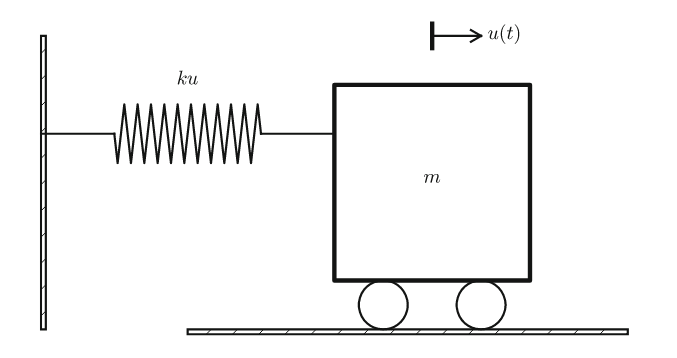
\includegraphics[width=0.9\textwidth]{Figures/Vibrating_system_scheme.png} % Example: scaled to 90% of the column width
		\vspace{0.2cm}
		\textbf{Example 1: Vibrating System}
		\vspace{0.3cm}
		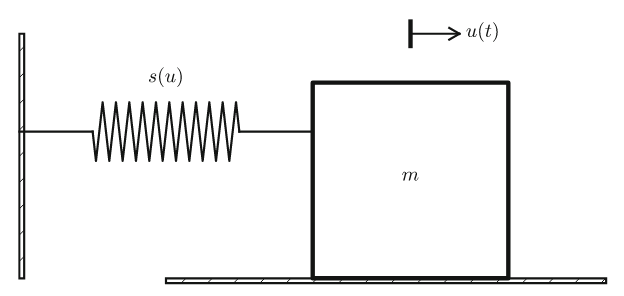
\includegraphics[width=0.8\textwidth]{Figures/Vibrating_sliding_system_scheme.png} % Example: scaled to 80% of the column width
		\vspace{0.2cm}
		\textbf{Example 3: Vibrating Sliding System}
	\end{minipage}
	\hfill
	\begin{minipage}[t]{0.48\textwidth}
		\centering
		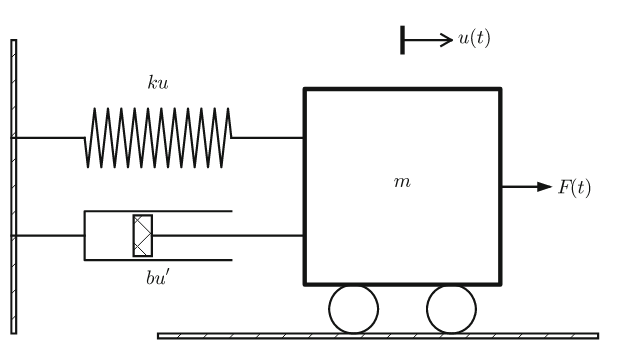
\includegraphics[width=1.0\textwidth]{Figures/Vibrating_dumped_system_scheme.png} % Example: scaled to full column width
		\vspace{0.2cm}
		\textbf{Example 2: Damped Vibrating}
		\vspace{0.3cm}
		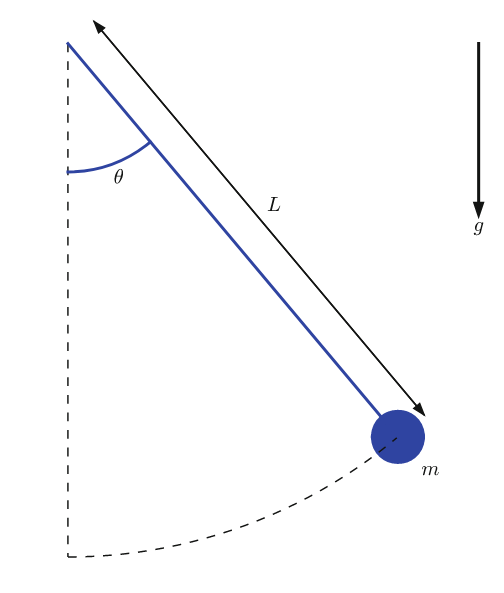
\includegraphics[width=0.5\textwidth]{Figures/simple_pendulum_scheme.png} % Example: scaled to 50% of the column width
		\vspace{0.2cm}
		\textbf{Example 4: Simple Pendulum System}
	\end{minipage}
\end{frame}

\begin{frame}{Open Sourcing of Code}
	\justifying
	\textbf{GitHub Repository:}
	\begin{itemize}
		\item Explore the code and examples at: \href{https://github.com/pb96git/Numerical-Solutions-for-Partial-Differential-Equations/tree/main}{\texttt{GitHub Repository Link}}
	\end{itemize}
\end{frame}


\end{document}